\documentclass{article}

% Language setting
% Replace `english' with e.g. `spanish' to change the document language
\usepackage[spanish]{babel}

% Set page size and margins
% Replace `letterpaper' with `a4paper' for UK/EU standard size
\usepackage[letterpaper,top=2cm,bottom=2cm,left=3cm,right=3cm,marginparwidth=1.75cm]{geometry}

% Useful packages
\usepackage{amsmath}
\usepackage{graphicx}
\usepackage[colorlinks=true, allcolors=blue]{hyperref}

\title{Practica 2 TALF}
\author{José Ruiz Pareja}

\begin{document}
\maketitle

Considera el lenguaje sobre el alfabeto {a, b} que solamente contiene la cadena
a: L = \{a\}.

\section{Autómata finito en JFLAP:}

\textbf{Construye un AFD que reconozca el lenguaje y rechace todas las cadenas que no pertenezca al lenguaje.}

\begin{center}
    \centering
    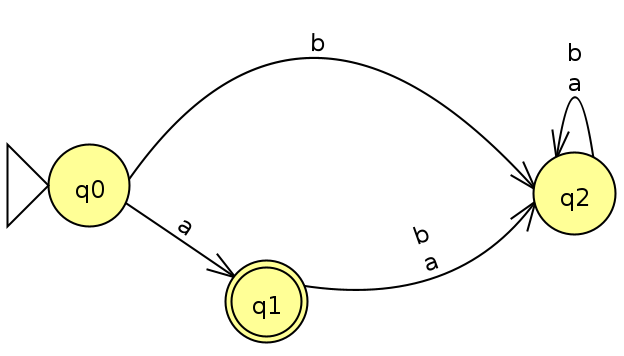
\includegraphics[width=0.5\linewidth]{automata1.png}
\end{center}

\textbf{Verifica el autómata construido con 6 cadenas de ejemplo.}


\begin{center}
    \centering
    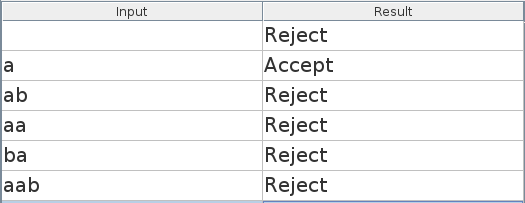
\includegraphics[width=0.5\linewidth]{CadenasEjemplo.png}
\end{center}

Observamos que el automata solo acepta la cadena \textit{a}, y rechaza el resto: $\{\varepsilon, ab, aa, ba, aab\}$


\newpage

\section{Autómata finito en Python:}

\textbf{Abre el módulo automata y crea en Python un autómata equivalente al construido en la actividad anterior mediante finite\_automaton.}

Añadimos a \textit{finiteautomata.json} el automata:
\begin{verbatim}
    {
    "name" : "solo_a",
    "representation" : {
      "K" : ["q0", "q1", "q2"],
      "A" : ["a", "b"],
      "s" : "q0",
      "F" : ["q1"],
      "t" : [["q0", "b", "q2"],
      	     ["q0", "a", "q1"],
             ["q1", "b", "q2"],
             ["q1", "a", "q2"],
             ["q2", "a", "q2"],
             ["q2", "b", "q2"]]
      }
  }
\end{verbatim}

\textbf{Ejecuta varias cadenas de prueba y comprueba cuáles son aceptadas.}

 \begin{center}
      \centering
      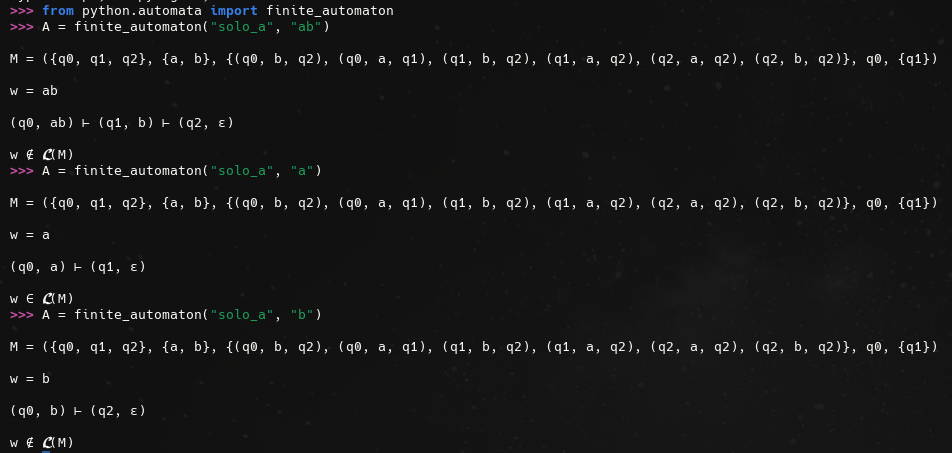
\includegraphics[width=0.75\linewidth]{cadenasPython.png}
  \end{center} 

Como podemos ver solo acepta la cadena $a$ y rechaza el resto de cadenas

\newpage

\section{Repite los pasos anteriores pero con un AFND y compara su comportamiento con el AFD.}

\textbf{Construye un AFND que reconozca el lenguaje y rechace todas las cadenas que no pertenezca al lenguaje. Verifica el autómata construido con 6 cadenas de ejemplo.}


\begin{center}
    \centering
    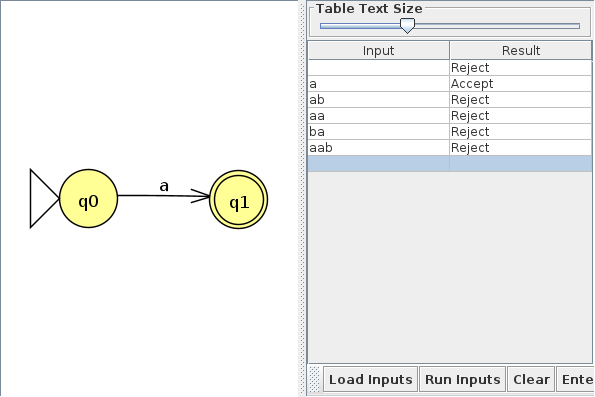
\includegraphics[width=0.6\linewidth]{automata2ycadenas.png}
\end{center}

\textbf{Crea en Python un autómata equivalente al construido en la actividad anterior mediante finite\_automaton y ejecuta varias cadenas de prueba y comprueba cuáles son aceptadas.}

\begin{verbatim}
{
    "name" : "solo_a_afnd",
    "representation" : {
      "K" : ["q0", "q1"],
      "A" : ["a", "b"],
      "s" : "q0",
      "F" : ["q1"],
      "t" : [["q0", "a", "q1"]]
      }
  }
\end{verbatim}

\begin{center}
    \centering
    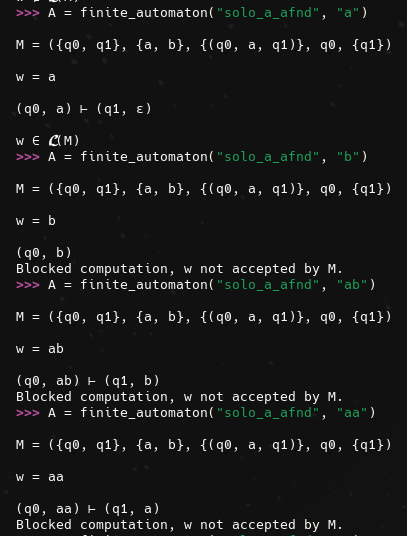
\includegraphics[width=0.45\linewidth]{cadenasPythonAFND.png}
    \label{fig:placeholder}
\end{center}

\end{document}
